\documentclass[a4paper,10pt]{article}
\usepackage[utf8]{inputenc}
\usepackage{amsmath}
\usepackage{amssymb}
\usepackage{graphicx}



\begin{document}

To begin, what is a moment? A moment is, quite simply, the expected value of a random variable, $z$, raised to a certain power. An ``expectation'' is a specifically defined function in statistics, $E\left[f(z)\right]=\int f(z) P(z) dz$ when in continuous spaces or $\sum f(z) P(z)$ in discrete spaces. In general, we can talk about the $i$th moment as:

$$ \mu_i (t) = E\left[ z^i \right] = \sum_{z=0}^\infty P(z,t) z^i$$

 A probability distribution is uniquely defined by its full set of moments, and sometimes it is more conveniant or informative to talk about a system's moments than the contour of its distribution. Having access to these moments could eliminate the need to solve for the full distribution, depending on what information would be considered important. A special function, called the Moment Generating Function, is specifically intended for this purpose:
$$M(\theta, t)=\sum_{z=0}^\infty e^{\theta z} P(z,t)$$
By taking the Taylor expansion of $e^{\theta z}=1 + \frac{(\theta z)^1}{1!}+\frac{(\theta z)^2}{2!}+\frac{(\theta z)^3}{3!}+\cdots$, we can see the moments emerging from this function, the $i$th moment associated with the $i$th power of $\theta$:
$$M(\theta, t)=\mu_0(t)+\frac{\mu_{1}(t)\theta}{1!}+\frac{\mu_{2}(t)\theta^2}{2!}+\cdots=\sum_{z=0}^\infty \frac{\mu_z(t)\theta^z}{z!}$$.

The following equations will be used extensively in the following derivation, so it will be useful to define them now:
\begin{align}
 M(\theta, t)&=\sum_{z=0}^\infty e^{\theta z} P(z,t)=\sum_{z=0}^\infty \frac{\mu_z(t)\theta^z}{z!}\\
 \frac{\partial M(\theta, t)}{\partial t} &=\sum_{z=0}^\infty e^{\theta z} \frac{\partial P(z,t)}{\partial t}\\
  \frac{\partial^i M(\theta, t)}{\partial \theta^i} &=\sum_{z=0}^\infty e^{\theta z} P(z,t)  z^i=\sum_{z=0}^\infty \frac{\mu_z(t)\theta^{z-i}}{(z-i)!}
\end{align}

\section{The Chemical Master Equation}
Since we will be uniquely considering the structure of the Chemical Master Equation, we would like to derive a general version of the Moment Generating Function which can be used for any system: we would simply have to plug in the specific values unique to that particular instance. The CME for $l$ reactions with stoichiometric change $v_l$ is:
$$\frac{\partial P(z,t|z_0,t_0)}{\partial t} = \sum_l a_l(z-v_l)P(z-v_l,t) - a_l(z)P(z,t)a$$
As we will see later on, the kind of rate laws associated with the system dramatically impact the complexity of the overall problem. We begin with the most simple case of kinetic mass action laws, following the derivation from \cite{1}. However, we would eventually like to take rational rate laws, such as Hill functions, as is seen in \cite{2}. An example of a mass action rate law is $a_l(z)= \frac{\lambda z_1(z_1-1)}{2}= \frac{\lambda}{2}z_1^2-\frac{\lambda}{2}z_1=\sum_i c_{l,i} a\prime_{l,i}$, where the law can be rewriten as a sum of coefficients $c_{l,i} $ and variables $a\prime_{l,i}$. This expanded, polynomial form will be exploited in our derivation.

Since we would like to talk about moments of the CME rather than probabilities, our first priority is to write this equation in terms of $M$, rather than in terms of $P$. We multiply both sides by $e^{\theta z}$ and sum over all possible values of $z$:
$$\sum_{z=0}^\infty e^{\theta z} \frac{\partial P(z,t)}{\partial t} = \sum_{z=0}^\infty \sum_l e^{\theta z} a_l(z-v_l)P(z-v_l,t) - e^{\theta z} a_l(z)P(z,t)$$
The left hand side is equivalent to equation (1). For the second right hand term, we see the beginnings of functions of $M$. However, we must account for the variables of $a_l(z)$, $a\prime_{l,i}(z)$, by taking equation (2), in which these variables will come out to the $i$th power with $i$ derivatives, $i=\{i_1\cdots i_N\}$.
\begin{align*}
 \frac{\partial M(\theta, t)}{\partial t} &= \sum_{z=0}^\infty \sum_l \sum_i c_{l,i} a\prime_{l,i}(z-v_l) e^{\theta z} P(z-v_l,t) - \sum_i c_{l,i} a\prime_{l,i}(z) e^{\theta z} P(z,t)  \\
 &= \sum_{z=0}^\infty \sum_l \sum_i c_{l,i} a\prime_{l,i}(z-v_l) e^{\theta (z-v_l)} e^{\theta (v_l)}P(z-v_l,t) - \sum_i c_{l,i} a\prime_{l,i}(z) e^{\theta z} P(z,t)  \\
  &=  \sum_l \sum_i c_{l,i} \frac{\partial ^i M}{\partial \theta^i} e^{\theta (v_l)} - \sum_i c_{l,i} \frac{\partial ^i M}{\partial \theta^i} \\
  &=  \sum_l \sum_i c_{l,i} \frac{\partial ^i M}{\partial \theta^i} \left(e^{\theta (v_l)}-1\right) 
\end{align*}

Now, we can take the second definition of $\frac{\partial ^i M}{\partial \theta^i}$ and expand $e^{\theta (v_l)}$ into its Taylor series. Notice that the summation, normally $\left[j=0\cdots \infty\right]$, now begins at $j=i$. When $j<i$, the index will be out of bounds and not correspond to any physical state.
\begin{align*}
 \frac{\partial M(\theta, t)}{\partial t} &= \sum_l \sum_i c_{l,i} \frac{\partial ^i M}{\partial \theta^i} \left(e^{\theta (v_l)}-1\right)\\
 &= \sum_l \sum_i c_{l,i} \sum_{j=i}^\infty \frac{\mu_j(t)\theta^{j-i}}{(j-i)!}\left(\sum_{k=0}^\infty \frac{{(\theta v_l)}^k}{k!}-1\right)
\end{align*}

Remember that the initial goal was to isolate the coefficients of $\theta^n$ in order to obtain the $n$th moments:
\begin{align*}
 \frac{\partial M(\theta, t)}{\partial t} &= \sum_l \sum_i c_{l,i} \sum_{j=i}^\infty \frac{\mu_j(t)\theta^{j-i}}{(j-i)!} \left( \sum_{k=0}^\infty \frac{{(\theta v_l)}^k}{k!}-1 \right)\\
&= \sum_l \sum_i c_{l,i} \left( \frac{\mu_i}{0!}+\frac{\mu_{i+1}\theta}{1!}+\frac{\mu_{i+2}\theta^2}{2!}+\cdots \right) \left(\frac{v_l \theta}{1!}+\frac{{(v_l \theta)}^2}{2!}+\frac{{(v_l \theta)}^3}{3!}+\cdots\right)\\
 &= \sum_l \sum_i c_{l,i} \left( \left[\frac{\mu_i}{0!}\frac{v_l}{1!}\right]\theta+\left[\frac{\mu_{i}}{0!}\frac{{v_l}^2}{2!}+\frac{\mu_{i+1}}{1!}\frac{{v_l}}{1!}\right]\theta^2+\left[\frac{\mu_{i}}{0!}\frac{{v_l}^3}{3!}+\frac{\mu_{i+1}}{1!}\frac{{v_l}^2}{2!}+\frac{\mu_{i+2}}{2!}\frac{{v_l}}{1!}\right]\theta^3+\cdots\right)\\
  &=\sum_l \sum_i c_{l,i} \sum_{n=0}^\infty \theta^n \sum_{k=1}^n \mu_{i+(n-k)} \frac{1}{k!(n-k)!}
\end{align*}
This is where my derivation separates from that of the paper, where the author has put $\frac{n!}{k!(n-k)!}$. I believe that the original paper contains an error. Our next step will be isolate just the coefficients of $\theta$ in order to achieve a form in which we are creating ODE's of $\mu$ rather than $M(\theta, t)$. Since $\frac{\partial M(\theta, t)}{\partial t}=\sum_n \frac{\partial \mu_n}{\partial t}\frac{1}{n!}\theta^n$, 
 we will have to multiply both sides by $n!$ in order to isolate $\mu$. Thus:
  $$ \frac{\partial \mu_n(t)}{\partial t}=\sum_l \sum_i c_{l,i} \sum_{k=1}^n v_l^k \mu_{i+(n-k)} \frac{n!}{k!(n-k)!}$$

  
 \section{Example}
 We will use the same example as found in the original paper, a reversible dimerisation with mass action rate laws. The system is as follows:
 \begin{align*}
  2X\rightarrow^{k1}Y\\
   Y\rightarrow^{k2}2X\\
 \end{align*}
 For convenience, we will only try to solve for moments in $X$, noting that $X_0= X-2Y$ is the total number of $X$ molecules, bound or unbound. To write the mass action laws for the two reactions is relatively simple. For the first reaction, two unique $X$ molecules must be chosen, noting that the combination is symmetric. The second only depends on the presence of $Y$, or $\frac{(X_0-X)}{2}$.
 \begin{align*}
   a_{1}&=\frac{k_1 X(X-1)}{2}\\
  a_{2}&=\frac{k_2 (X_0-X)}{2}
 \end{align*}
The coefficients can then be isolated:
$$ c_{l,i}=\begin{cases}
                  &l=1,i=1: \frac{-k_1}{2}\\
                  &l=1,i=2: \frac{k_1}{2}\\
                  &l=2,i=0: \frac{k_2 X_0}{2}\\
                   &l=1,i=1: \frac{-k_2}{2}\\
                 \end{cases}$$
We also know the stoichiometric changes. The first reaction will cause the system to loose two $X$, $v_1=-2$, and the second to gain them back $v_2=2$. Now, we only have to plug these values into our equations for the first and second moments. It should be noted that the ``zero'' moment, $\mu_0$ is the summation of all probabilities, or $1$.

\begin{align*}
 \frac{\partial \mu_1(t)}{\partial t}&=\sum_l \sum_i c_{l,i} v_l \mu_{i}\\
 &= c_{1,0}v_1\mu_0+c_{1,1}v_1\mu_1+c_{1,2}v_1\mu_2+c_{2,0}v_2\mu_0+c_{2,1}v_2\mu_1+c_{2,2}v_2\mu_2\\
 &= \frac{-k_1}{2}(-2)\mu_1 +\frac{k_1}{2}(-2)\mu_2+\frac{k_2 X_0}{2}(2)\mu_0+\frac{-k_2}{2}(2)\mu_1\\
 &= k_1(\mu_1-\mu_2)+k_2(X_0 - \mu_1)
\end{align*}

\begin{align*}
 \frac{\partial \mu_2 (t)}{\partial t} &= \sum_l \sum_i c_{l,i} \sum_{k=1}^2 v_l^k \mu_{i+(2-k)} \frac{2!}{k!(2-k)!}\\
 &=\sum_l \sum_i c_{l,i} \left[ v_l \mu_{i+1} \frac{2!}{1!1!}+v_l^k \mu_{i} \frac{2!}{2!0!}\right]\\
 &= c_{1,1}(v_l \mu_{2} 2!+v_l^2 \mu_1)+c_{1,2}(v_l \mu_{3} 2!+v_l^2 \mu_2)+c_{2,0}(v_l \mu_{1} 2!+v_l^2 \mu_0)+c_{2,1}(v_l \mu_{2} 2!+v_l^2 \mu_1)\\
 &= \frac{-k_1}{2}(-4\mu_2+4\mu_1)+\frac{k_1}{2}(-4\mu_3+4\mu_2)+\frac{k_2 X_0}{2}(4\mu_1+4\mu_0)+\frac{-k_2}{2}(4\mu_2+4\mu_1)\\
 &=2k_1(-\mu_1+2\mu_2-\mu_3)+2k_2(X_0+(X_0-1)\mu_1-\mu_2)
\end{align*}
 
 As we can see, each moment depends on some moments higher than itself. In order to solve a system of ordinary differential equations, we will need to obtain an equation for $\mu_3$, which will, in turn, call for an equation for $\mu_4$, etc. Since there are an infinite number of moments, we cannot continue this process. In order to make the problem approachable, we must \textit{close} the chain of dependence by creating relationships between the moments. 
 
 \section{Moment Closure Relationships}
 
 We must make some kind of assumption about the distribution of our system in order to advance in the problem. Some schemes, for example, assume that the standard deviation is very small compared to the mean, or the inverse. Others imagine that the system exists in a very large volume with large molecule counts. However, the most common closure schemes simply impose a particular distribution type on the data. In this case, it is sometimes easier to talk in terms of \textit{cumulants}, or arithmetic combinations of moments which are sometimes more informative than the raw moments themselves. 
 
 \begin{align*}
  \kappa_1 &= \mu_1 \\
  \kappa_2 &= \mu_2 - \mu_1^2 \\
  \kappa_3 &= \mu_3 - 3\mu_1\mu_1+2\mu_1^3
 \end{align*}
It is these cumulants, and not their raw moments, which most people are familiar with and are most used in analysis of biological systems. For example, for a normal distribution, the second cumulant is called the variance, the third skew, and the fourth kurtosis. Since Gaussian distributions are symmetric about their mean, cumulants from the third and onward are equal to zero, creating a very simple means of writing the third cumulant as a function of the first two. Here, we have performed three of the most common distribution matching moment closures: normal ( $\mu_3 = 3\mu_1\mu_1-2\mu_1^3$), Poisson ($\mu_3=\mu_1+3\mu_1^2+\mu_1^3$), and log normal ($\mu_3=\frac{\mu_2}{\mu_1}^3$). Note that all of these closures attempt to stop the moment dependence at the same point: the third raw moment. This is known as the ``second order moment approximation'', or 2MA, and is widely used in the literature as the most direct path to the relevant information of the system: two desired moments, two differential equations. However, it is to be noted that \cite{3} recently proved that at least three moments, or the 3MA, is needed under certain closure schemes to provide accurate results. Here, we will continue to work with the 2MA, given the simplicity of the biochemical system at hand.
\begin{figure}[h!]
 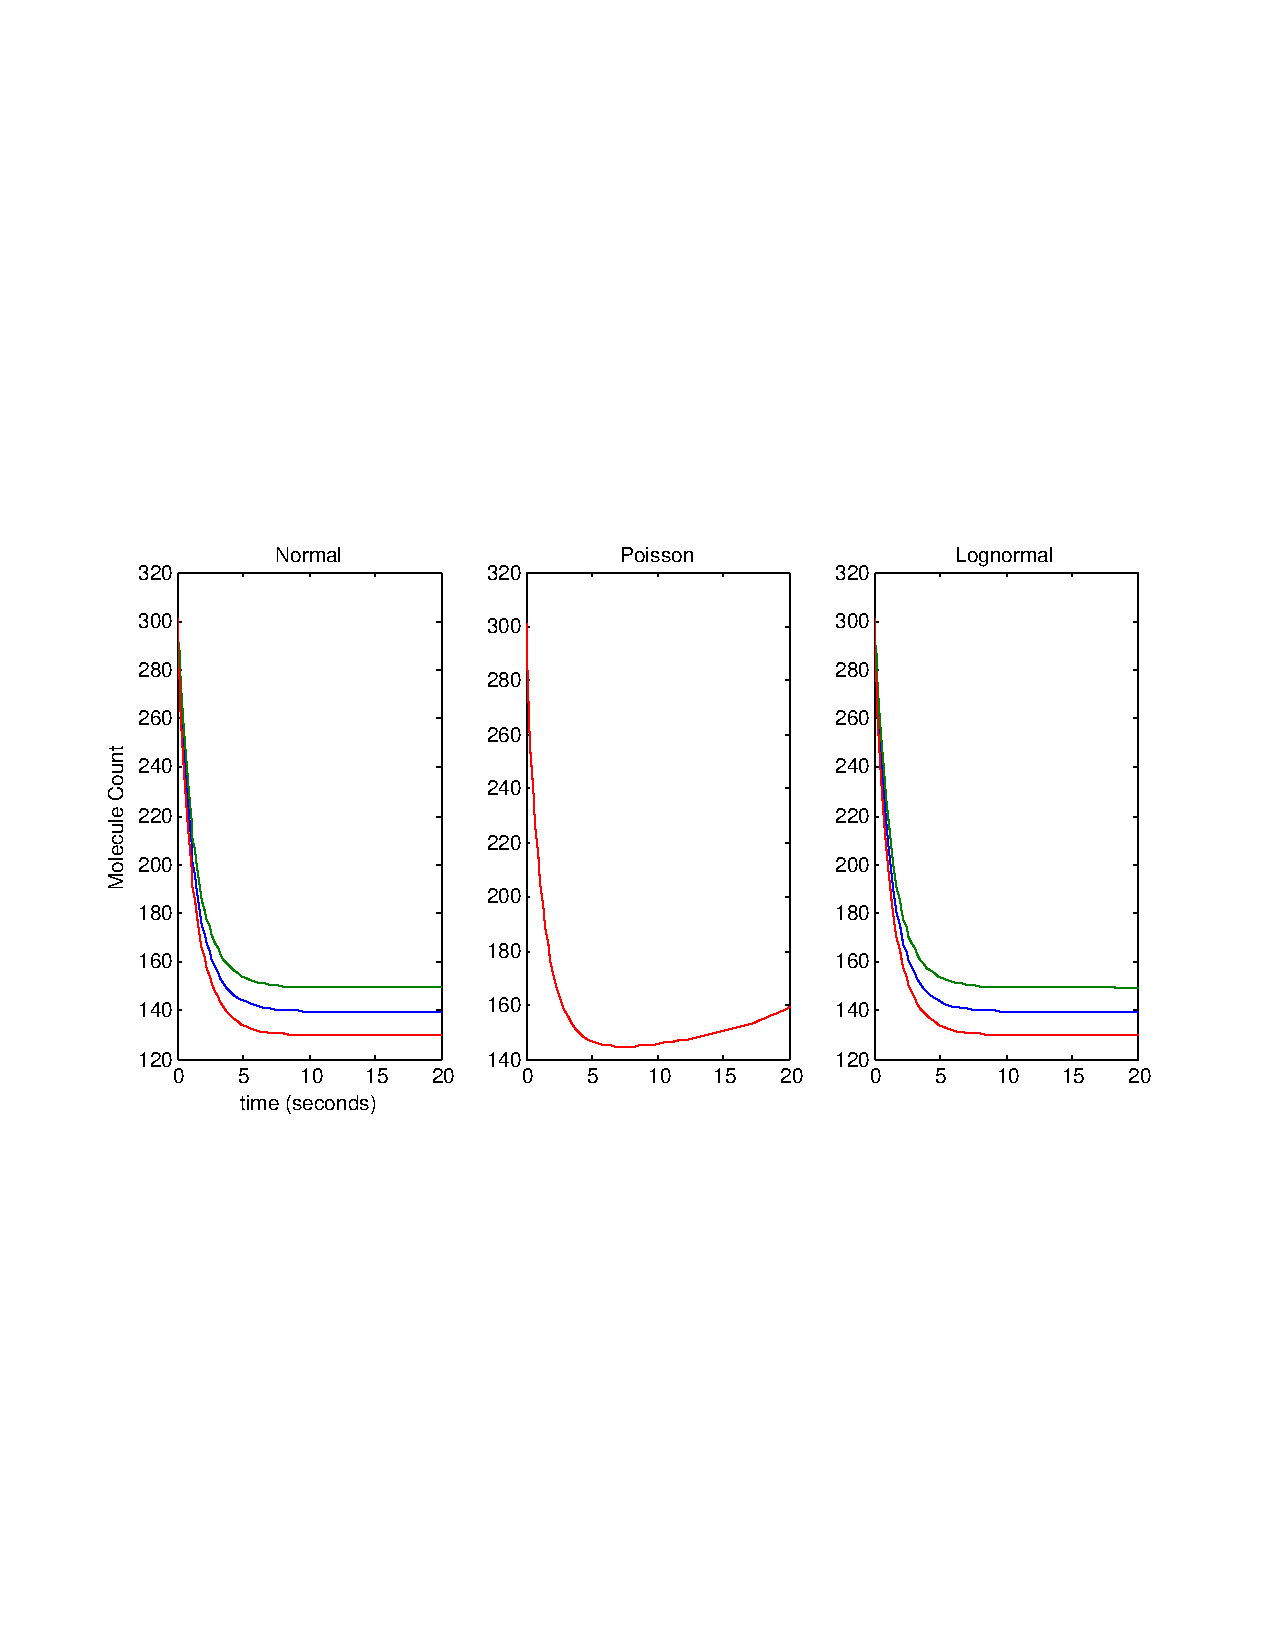
\includegraphics[width=\textwidth,height=.7\textwidth]{three_fits.pdf}
 \caption{Results from three distribution fitting closure schemes, normal, Poisson, and log normal, for their mean plus and minus one standard deviation. These figures suggest that the normal distribution may, in fact, be a good match for the data itself, especially when we compare our results to the ``true'' cumulants in Figure  \ref{true}.}
 \label{threefit}
\end{figure}
In order to know whether these results are accurate, however, we must have something to compare them to. Since the chosen dimerisation system is so simple, we may return to the Chemical Master Equation notation which we have been trying so hard to avoid! The CME is directly solvable, resulting in the probability distribution shown in Figure \ref{true}. To obtain the moments from this PDF, we can use the most simple definition available: $\mu_i=\sum_{z=0}^\infty P(z,t) z^i$. As we can see, both the normal and log normal closure schemes perform fairly well.
\begin{figure}[h!]
 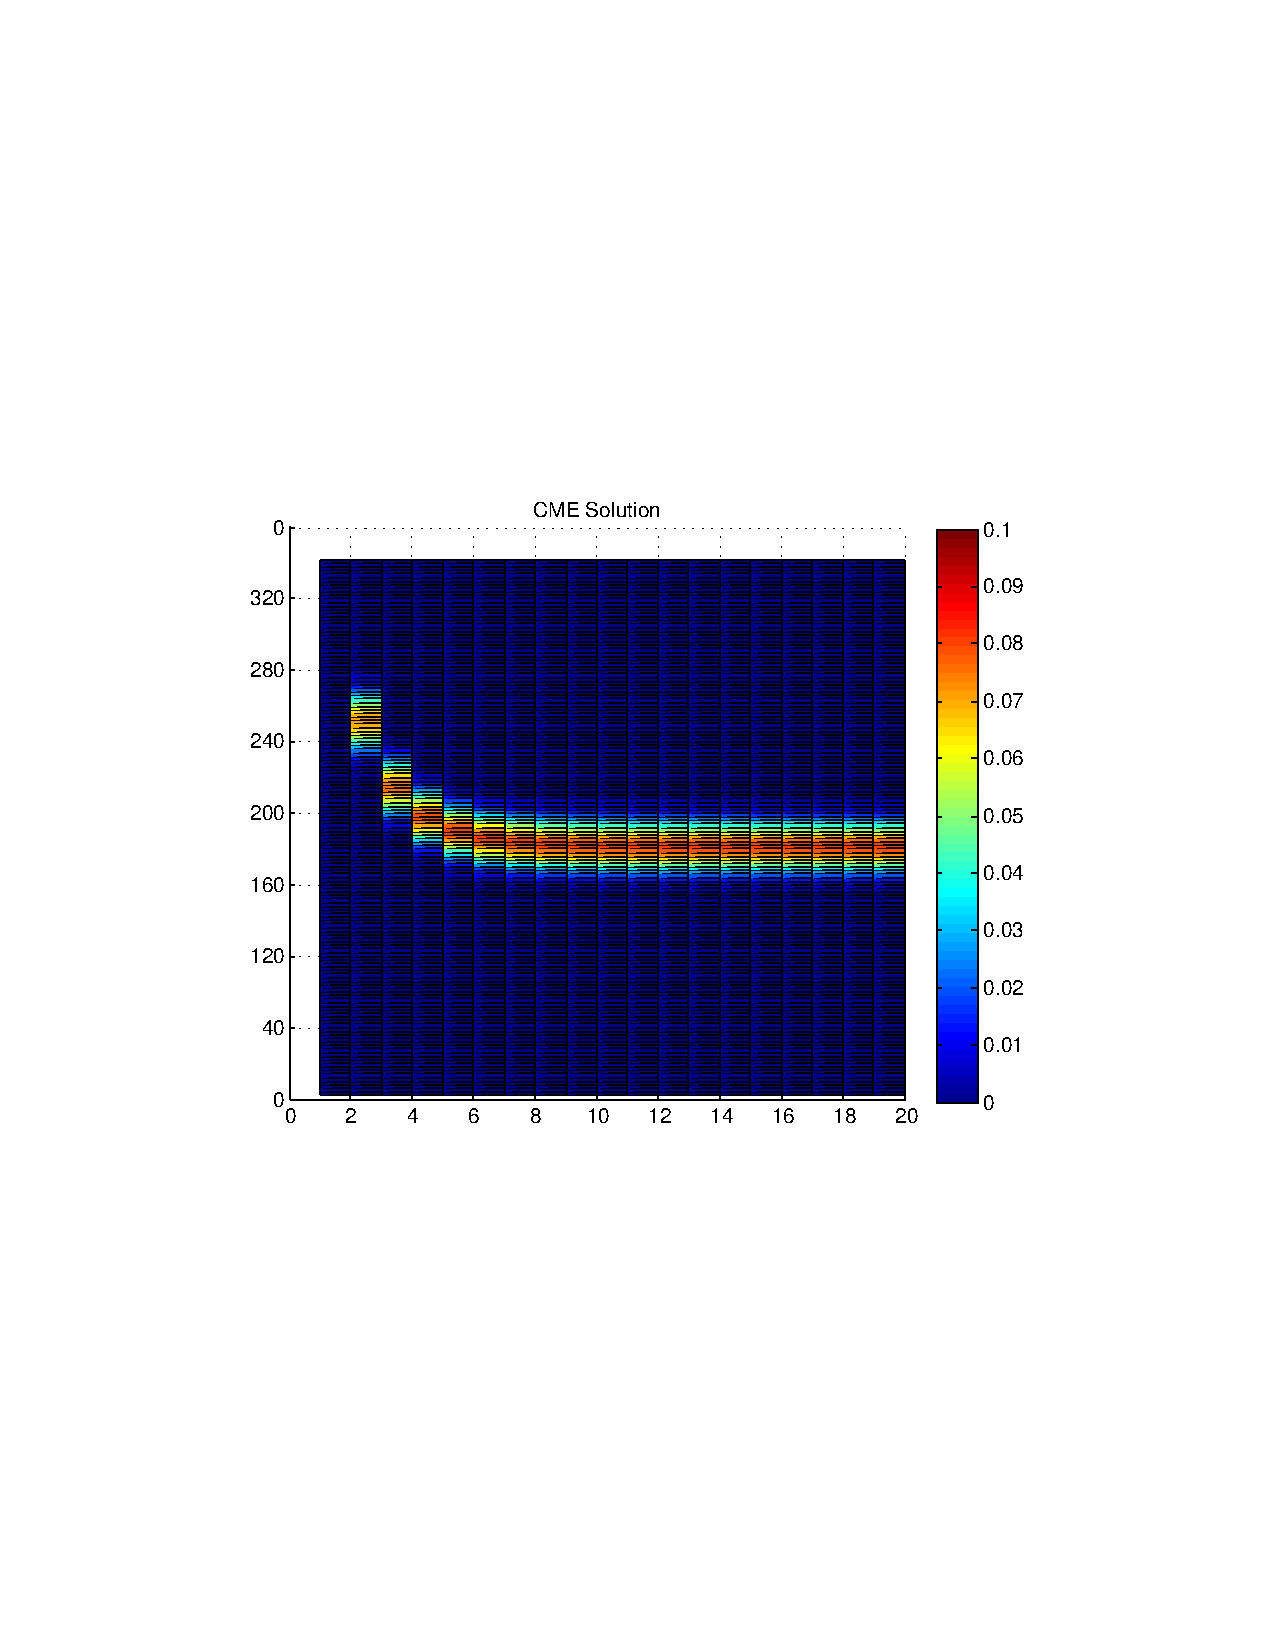
\includegraphics[width=\textwidth,height=\textwidth]{cme_solution.pdf}
 \caption{Results from directly solving the Chemical Master Equation associated with the dimerisation system illustrated in the previous section, shown here in 2D. From this distribution, we can directly extract the raw moments for the system, and thus the cumulants.}
 \label{true}
\end{figure}

\subsection{Arbitrary Closure Schemes}
Given the nature of biochemical systems, imposing a particular distribution form for all times is not a sound approach to obtaining moments as they evolve through time. We would like to consider arbitrary probability distributions, without any restrictions to shape which exclude skewed or multi-modal phenomena. With this in mind, we would like to make some first steps in creating unbiased closure schemes which are informed by the data itself rather than assumptions about its distribution shape. \\

From the Chemical Master Equation solution, shown in Figure \ref{true}, we are able to directly obtain all of the raw moments of the system, $\mu_1$, $\mu_2$, $\mu_3$, etc. Since we are taking on 2MA schemes, we wish to write the third moment as some function of the first two, $\mu_3=f\left(\mu_1, \mu_2\right)$. The most simple case is that when $f$ is a polynomial, for which we will only consider a handful of linear and nonlinear terms:
$$f\left(\mu_1, \mu_2\right)= c_1 \mu_1+c_2 \mu_1^2+c_3 \mu_1^3+c_4 \mu_2+c_5 \mu_2^2+c_6\mu_2^3+ c_7 \mu_1 \mu_2 + c_8\mu_1^2 \mu_2 +c_9\mu_1 \mu_2^2 $$
The coefficients to this polynomial can be fitted using the CME solution, taking each solution in time as a snapshot, the ensemble of which satisfies $\mu_3=F\left(\mu_1, \mu_2\right)*c$, where $F$ is the matrix of moment combinations throughout time and $c$ contains the coefficients of the polynomial. A ``best fit'' solution of $c$ can be obtained via linear least squares: $\hat{c}=inv\left(F^TF\right) F^T \mu_3$. The result is a moment closure scheme informed purely by the system itself. \\

However, this closure was taken for a given set of reaction rate parameters, $k_1=0.0166$ and $k_2=0.2$, and initial condition $X_0=301$. While it is most certainly well informed in this particular case, it is not obvious that this same closure scheme will be true for different parameters which change the overall dynamics of the system, or for which the probability distribution is a function of states and parameters, $\Phi(X,k_1,k_2)$. However, when we apply the polynomial closure scheme $\mu_3=f\left(\mu_1, \mu_2\right)$ with varying parameters, we see that the overall fit remains relatively good, with some special behaviors manifesting themselves as the rate parameters approach zero, see Figure \ref{errors}. Also noteworthy is the fact that the error seems to be a scaled function over a particular parameter, in this case, a function of $k_2$ which is simply scaled for values of $k_1$. If this is present in other biochemical systems, closures could be corrected by scaling terms according to the relationship between the parameters themselves.
\begin{figure}[h!]
 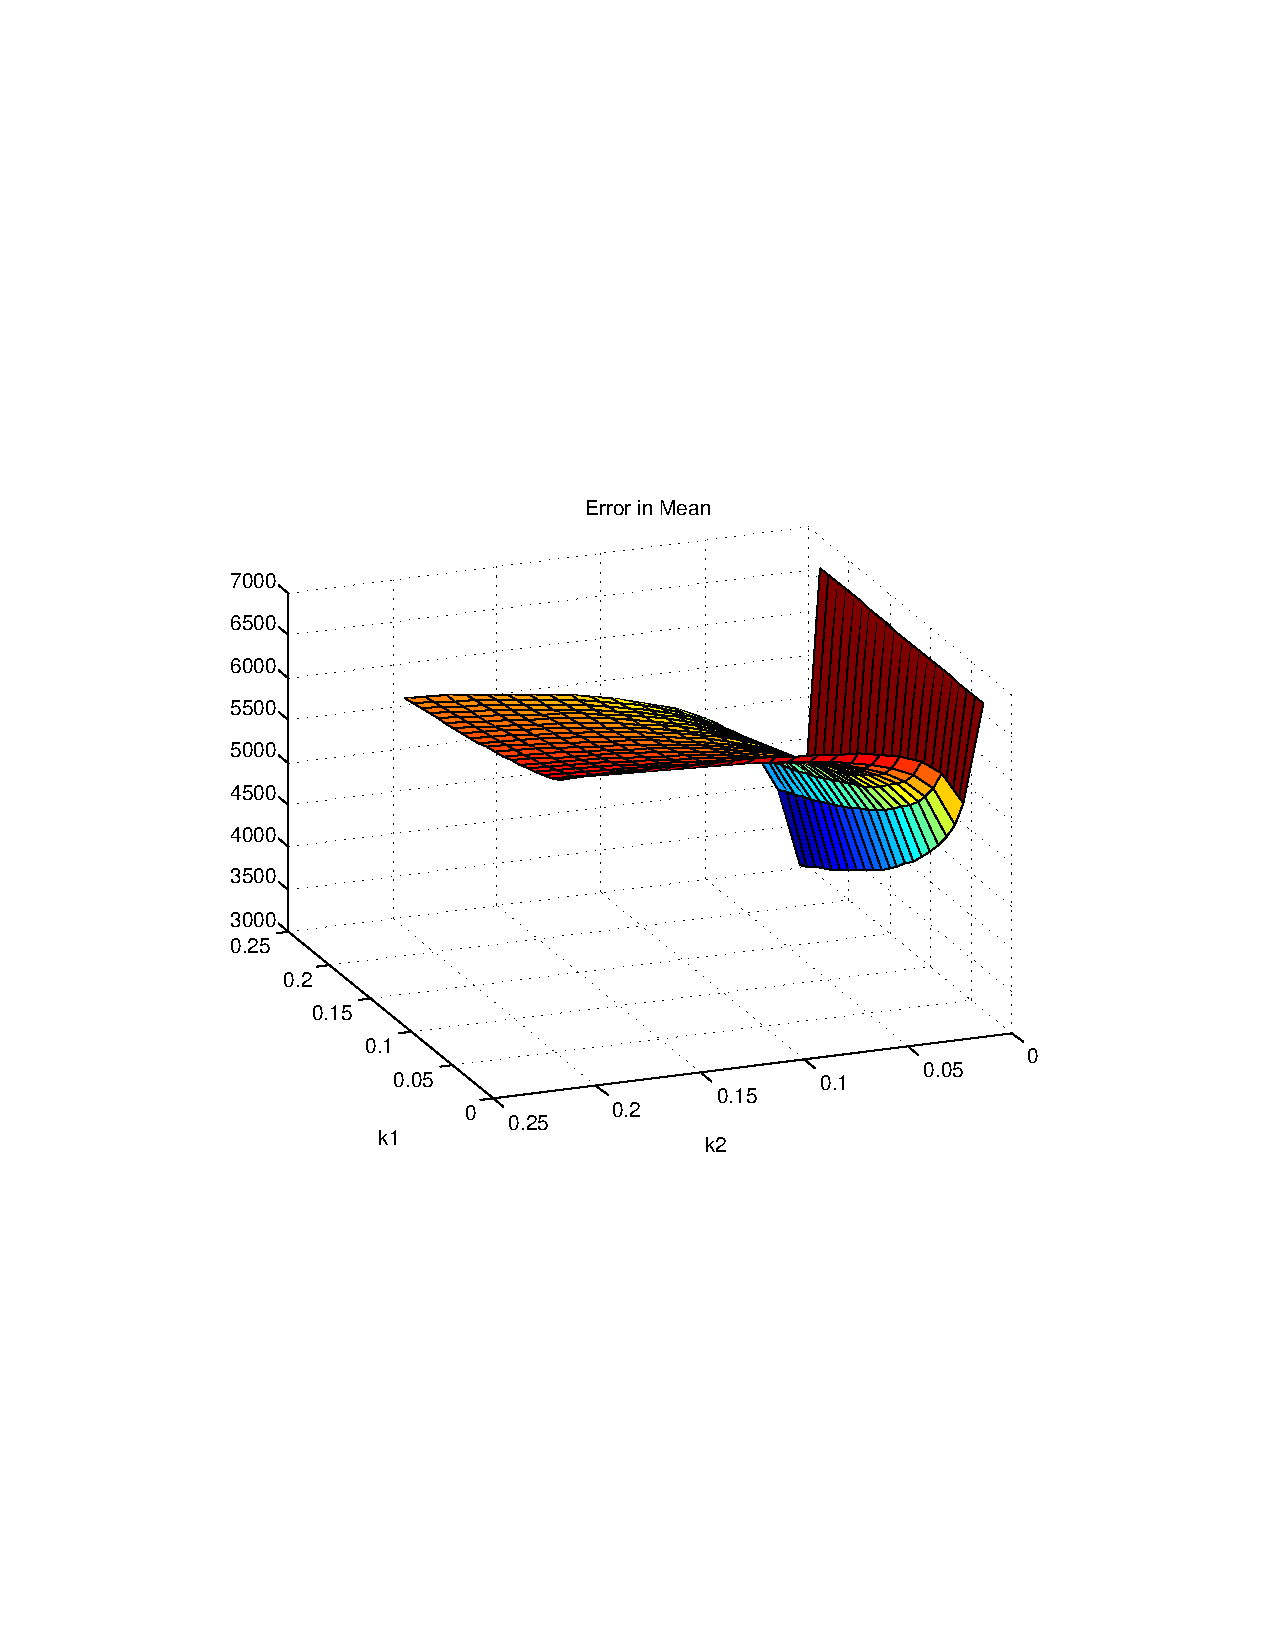
\includegraphics[width=.5\textwidth,height=.5\textwidth]{mean_errpr.pdf}
  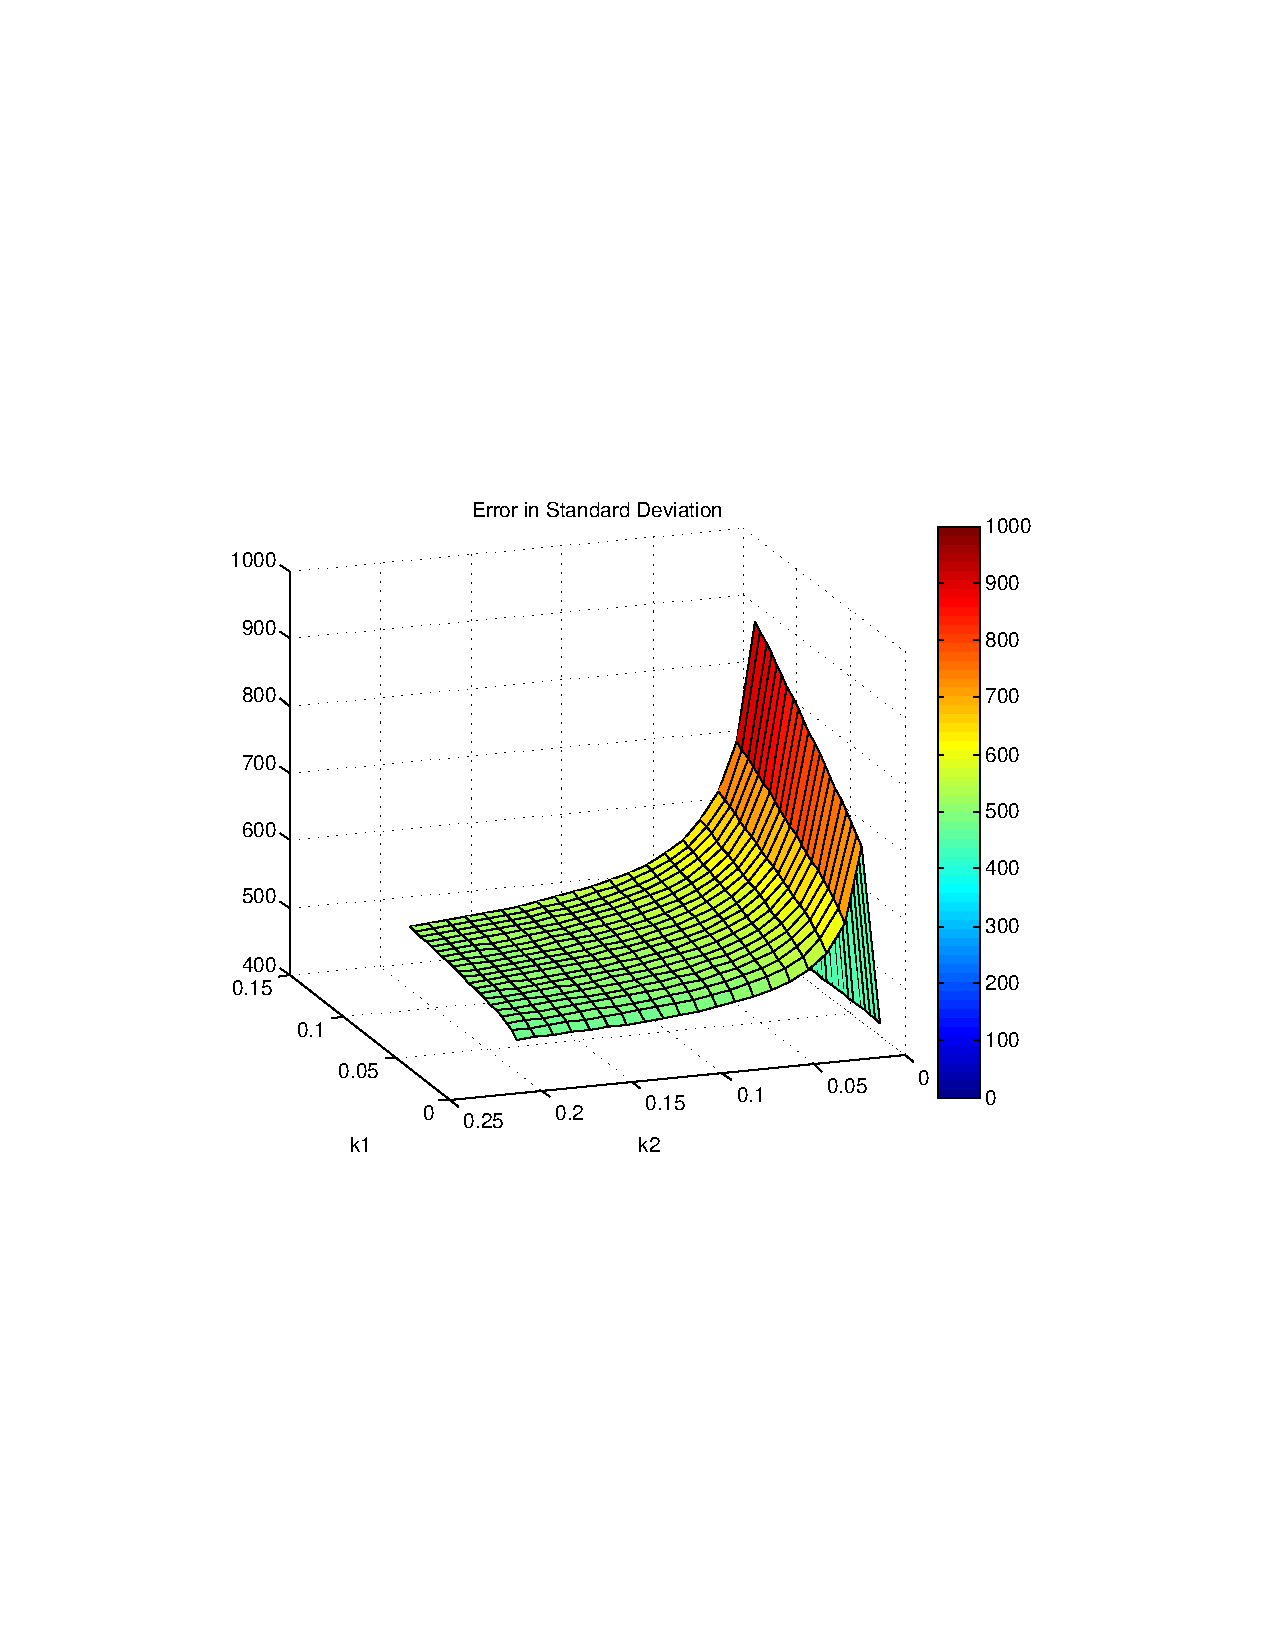
\includegraphics[width=.5\textwidth,height=.5\textwidth]{std_error.pdf}
 \caption{Errors in mean (right) and standard deviation (left) for multiple parameter sets. Special behaviors present themselves when $k_2$, or the rate for the reverse reaction, tends to zero. There seems to be an inverse relationship in the fit for mean and variance.}
 \label{errors}
\end{figure}
Given these first results, a potential work flow could go as follows:
For any given system
\begin{itemize}
 \item Approximate Chemical Master Equation solution, using PGD, for example, to fit polynomial closure schemes for only one set of parameters
 \item Use this closure scheme to obtain results for any set of parameters
 \item Include corrections to scale error down to minimum
\end{itemize}

\section{Looking Forward on Moment Closure as Applied to BioInformatics}
Now that we have explored Moment Closure, both in a literature review and in practice, I believe that it is appropriate to take a wider perspective on its potential as a numerical and analysis tool in the field of bioinformatics. My opinion in this matter is twofold in that I see a large potential for biochemical networks but remain unconvinced for genetic regulatory networks. \\

For biochemical networks, that is, networks which can be expressed in terms of stoichiometric reactions, the results seem promising. In the case of polynomial (mass action) rate laws, the construction of the differential equations themselves are relatively straightforward and have been automated in a Matlab toolbox illustrated in \cite{3} and a SBML/Python library illustrated in \cite{1}. Several potential applications of the work flow outlined in the previous section are possible, although, in my option, one of the most interesting is in simulation. Decomposition of a system into fast, deterministic reactions and slow, stochastic Markov events is relatively common. However, by representing the deterministic portion by moments, we are able to maintain the stochastic nature of the reactions while still being able to quickly produce accurate solutions in intermediate time scales. Results for systems of rational rate laws are still unsure: in \cite{2}, the authors conclude that the very form of the differential equations produced by the moment generating function may be impossible to solve as the number of interacting species grows: for example, for the first moment of a system of $N$ species, we obtain a single differential equation with $N$ unknowns. Moreover, it is not clear in the literature how well moment closure performs in the context of multi-modal  or oscillating systems, a crucial element of biological regulation.\\

Gene Regulatory Networks, however, are more precarious: not only are all reactions represented by rational rate laws (Hill or sigmoidal functions) and often dependent on multi-modal or oscillating dynamics, but the very structure of the system may prohibit a representation by moments, especially if we consider a discrete syntax. While it is true that the CME is discrete in that species are taken in the form of whole number molecule counts, the notion of its probability distribution remains relatively unchanged as this distribution is always a multivariate: each species receives one mean, for example, over the full extent of its possible values. However, discrete, qualitative networks are represented by a Bernoulli distribution. This means that each species is truly represented by a certain number of sub levels, each of which requires its own set of moments which are dependent not only on one another, but also on the sub levels of other connected species. This dependency may lead to an exponential explosion such that the very production of differential moment equations is impossible. \\

As a whole, I do not see Moment Closure as a sound approach to qualitative networks. If I continue on this same path for the remainder of my thesis, I will need to create stronger ties to qualitative networks, either by considering hybrid Boolean-differential systems or hybrid differential-stochastic systems. This alone, however, I do feel is a significant and interesting avenue if we choose to take it. Else, I feel as though this work somewhat deviates from the original efforts, all of which were focused around qualitative systems, especially Process Hitting. That said, I am interested in hearing your options about this research at our next meeting!

 \begin{thebibliography}{}
 \bibitem{1}	Gillespie, Colin S. "Moment-closure approximations for mass-action models." IET systems biology 3.1 (2009): 52-58.
\bibitem{2} Milner, Peter, Colin S. Gillespie, and Darren J. Wilkinson. "Moment closure approximations for stochastic kinetic models with rational rate laws." Mathematical biosciences 231.2 (2011): 99-104.
\bibitem{3} Hespanha, Joao. "Moment closure for biochemical networks." Communications, Control and Signal Processing, 2008. ISCCSP 2008. 3rd International Symposium on IEEE. (2008): 142-147.
\end{thebibliography}
 
 \end{document}
